% fig_pott_coverage.tex
% TR-33: Coverage map on (alpha, k_ibr) plane
% Shows TR-29 regions A/B/C/D and how POTT recovers Region B
%
% X-axis: k_ibr [0, 0.22] pu
% Y-axis: alpha [0, 1.10]
%
% Regions (same as TR-29 Fig 3, now annotated with POTT):
%   Region A: k_ibr < 0.10 (21 blocked; 87L sole detector)  — hatched gray
%   Region B: k_ibr >= 0.10, alpha > 0.80 (Zone 2 only)     — was red/fail, now green/POTT
%   Region C: k_ibr in [0.10,0.12), alpha <= 0.80             — blue/Zone1+TDCS
%   Region D: k_ibr >= 0.12, alpha <= 0.80                    — teal/Zone1+87L
%   Out: alpha > X_R2/Z1L = 1.20 (beyond Zone 2)
%
% alpha boundary: X_R1/Z1L = 0.80
% alpha_Z2 boundary: X_R2/Z1L = 1.20 (beyond Z2 reach)

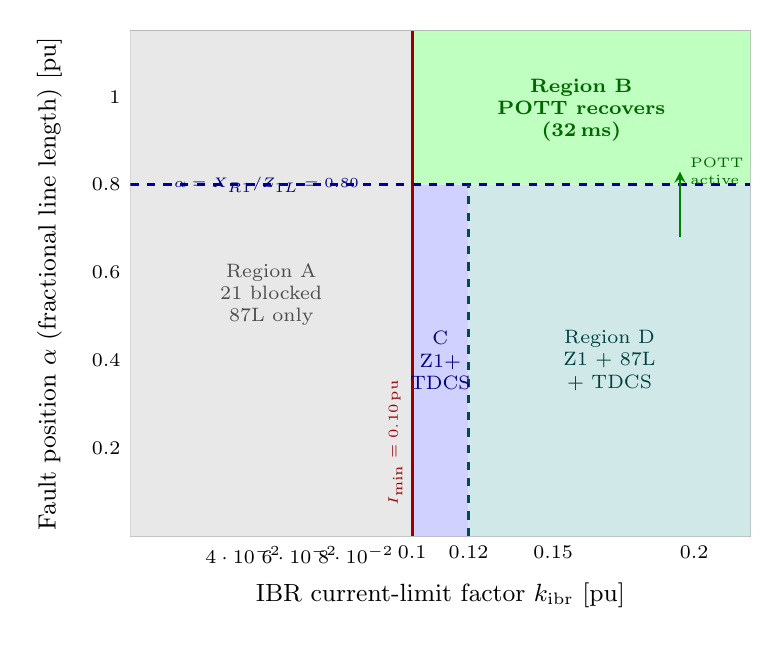
\begin{tikzpicture}[
  every node/.style = {font=\scriptsize},
]
\begin{axis}[
  name        = covax,
  width       = 0.78\textwidth,
  height      = 8.0cm,
  xlabel      = {IBR current-limit factor $k_\mathrm{ibr}$ [pu]},
  ylabel      = {Fault position $\alpha$ (fractional line length) [pu]},
  xlabel style= {font=\small},
  ylabel style= {font=\small, yshift=4pt},
  xmin=0.0, xmax=0.22,
  ymin=0.0, ymax=1.15,
  xtick       = {0.04,0.06,0.08,0.10,0.12,0.15,0.20},
  ytick       = {0.20,0.40,0.60,0.80,1.00},
  xticklabel style={font=\scriptsize},
  yticklabel style={font=\scriptsize},
  grid        = major,
  grid style  = {gray!12, dashed},
  tick style  = {draw=none},
  axis line style={gray!60},
]

%% ── Region A: k_ibr < 0.10 (all alpha) — 21 blocked ─────────────────────────
\addplot[fill=gray!18, draw=none, area legend]
  coordinates {(0,0) (0.10,0) (0.10,1.15) (0,1.15)} \closedcycle;

%% ── Region B: k_ibr >= 0.10, alpha > 0.80 — POTT (was failing) ──────────────
\addplot[fill=green!25, draw=none]
  coordinates {(0.10,0.80) (0.22,0.80) (0.22,1.15) (0.10,1.15)} \closedcycle;

%% ── Region C: k_ibr in [0.10,0.12), alpha <= 0.80 — Zone1+TDCS ──────────────
\addplot[fill=blue!18, draw=none]
  coordinates {(0.10,0) (0.12,0) (0.12,0.80) (0.10,0.80)} \closedcycle;

%% ── Region D: k_ibr >= 0.12, alpha <= 0.80 — Zone1+87L ──────────────────────
\addplot[fill=teal!18, draw=none]
  coordinates {(0.12,0) (0.22,0) (0.22,0.80) (0.12,0.80)} \closedcycle;

%% ── Region boundary lines ─────────────────────────────────────────────────────
% k_ibr = I_min = 0.10 (vertical, Region A boundary)
\addplot[red!60!black, very thick, mark=none]
  coordinates {(0.10, 0) (0.10, 1.15)};

% alpha = 0.80 (horizontal, Z1/Z2 boundary)
\addplot[blue!60!black, very thick, mark=none, dashed]
  coordinates {(0.0, 0.80) (0.22, 0.80)};

% k_ibr = 0.12 (vertical, C/D boundary)
\addplot[teal!60!black, thick, mark=none, dashed]
  coordinates {(0.12, 0.0) (0.12, 0.80)};

%% ── Region labels ────────────────────────────────────────────────────────────
\node[gray!60!black, align=center, font=\scriptsize]
  at (axis cs:0.05, 0.55) {Region A\\21 blocked\\87L only};

\node[green!40!black, align=center, font=\scriptsize\bfseries]
  at (axis cs:0.16, 0.97)
  {Region B\\POTT recovers\\(32\,ms)};

\node[blue!50!black, align=center, font=\scriptsize]
  at (axis cs:0.11, 0.40) {C\\Z1+\\TDCS};

\node[teal!50!black, align=center, font=\scriptsize]
  at (axis cs:0.17, 0.40) {Region D\\Z1 + 87L\\+ TDCS};

%% ── I_min threshold label ────────────────────────────────────────────────────
\node[red!60!black, font=\tiny, above=2pt, rotate=90]
  at (axis cs:0.10, 0.20) {$I_\mathrm{min}=0.10$\,pu};

%% ── alpha = 0.80 label ────────────────────────────────────────────────────────
\node[blue!50!black, font=\tiny, right=2pt]
  at (axis cs:0.01, 0.80) {$\alpha=X_{R1}/Z_{1L}=0.80$};

%% ── POTT arrow annotation ────────────────────────────────────────────────────
\draw[->, >=stealth, green!50!black, thick]
  (axis cs:0.195, 0.68) -- (axis cs:0.195, 0.83)
  node[right, font=\tiny, green!40!black, align=left] {POTT\\active};

\end{axis}
\end{tikzpicture}
